%!TEX TS-program = xelatex
%!TEX encoding = UTF-8 Unicode

\documentclass[11pt,tikz,border=1]{standalone}
\usetikzlibrary{calc,positioning}

\usepackage{fontspec}
% file: westernfonts.tex

\newfontfamily\SourceCodePro{SourceCodePro}[
  UprightFont=*-Light,
  BoldFont=*-Medium,
  ItalicFont=*-LightIt,
  BoldItalicFont=*-MediumIt]

\newfontfamily\SourceSerifPro{SourceSerifPro}[
  UprightFont=*-Light,
  BoldFont=*-Semibold]

\newcommand{\serif}[0]{\SourceSerifPro}
 
\setmonofont{SourceCodePro}[
  UprightFont=*-Light,
  BoldFont=*-Medium,
  ItalicFont=*-LightIt,
  BoldItalicFont=*-MediumIt]


\begin{document}
  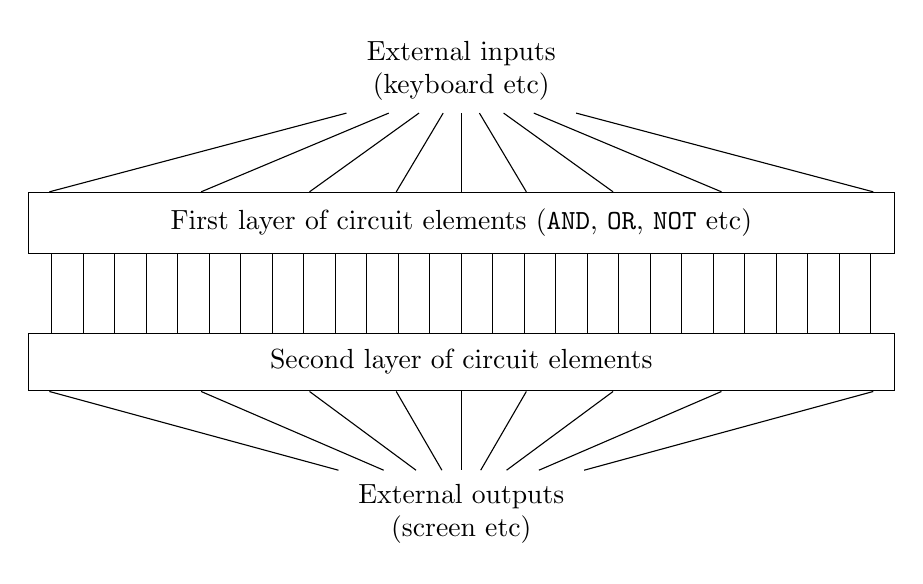
\begin{tikzpicture}[font={\RobotoLight}]

    \foreach \x in {0,...,26}
      \draw (\x * 0.4,0) -- (\x * 0.4, 1);

    \coordinate (layer1bottom) at (5.2,1);
    \coordinate (layer2top) at (5.2,0);
    \node(layer1) [above,rectangle,draw,minimum width=11cm,inner sep=6pt] at (layer1bottom) {
      First layer of circuit elements (\texttt{AND}, \texttt{OR}, \texttt{NOT} etc)
    };

    \node(layer2) [below,rectangle,draw,minimum width=11cm,inner sep=6pt] at (layer2top) {
      Second layer of circuit elements
    };
    
    \node(input) [above=of layer1] {
      \begin{tabular}{c}
        External inputs\\
        (keyboard etc)
      \end{tabular}
    };
    
    \node(output) [below=of layer2] {
      \begin{tabular}{c}
        External outputs\\
        (screen etc)
      \end{tabular}
    };

    \coordinate (t0) at (layer1.north);
    \coordinate (t1) at (layer1.north east);
    \coordinate (t2) at (layer1.north west);
    \coordinate (i0) at (input.south);
    \coordinate (i1) at (input.south east);
    \coordinate (i2) at (input.south west);
    
    \draw (i0) to (t0);
    \foreach \x in {0.15,0.35,0.6,0.95}
      \draw ($ (i0)!\x!(i1) $) to ($ (t0)!\x!(t1) $);
    \foreach \x in {0.15,0.35,0.6,0.95}
      \draw ($ (i0)!\x!(i2) $) to ($ (t0)!\x!(t2) $);

    \coordinate (b0) at (layer2.south);
    \coordinate (b1) at (layer2.south east);
    \coordinate (b2) at (layer2.south west);
    \coordinate (o0) at (output.north);
    \coordinate (o1) at (output.north east);
    \coordinate (o2) at (output.north west);

    \draw (b0) to (o0);
    \foreach \x in {0.15,0.35,0.6,0.95}
      \draw ($ (b0)!\x!(b1) $) to ($ (o0)!\x!(o1) $);
    \foreach \x in {0.15,0.35,0.6,0.95}
      \draw ($ (b0)!\x!(b2) $) to ($ (o0)!\x!(o2) $);

  \end{tikzpicture} 
\end{document}
